\documentclass[11pt,preprint, authoryear]{elsarticle}

\usepackage{lmodern}
%%%% My spacing
\usepackage{setspace}
\setstretch{1.2}
\DeclareMathSizes{12}{14}{10}{10}

% Wrap around which gives all figures included the [H] command, or places it "here". This can be tedious to code in Rmarkdown.
\usepackage{float}
\let\origfigure\figure
\let\endorigfigure\endfigure
\renewenvironment{figure}[1][2] {
    \expandafter\origfigure\expandafter[H]
} {
    \endorigfigure
}

\let\origtable\table
\let\endorigtable\endtable
\renewenvironment{table}[1][2] {
    \expandafter\origtable\expandafter[H]
} {
    \endorigtable
}


\usepackage{ifxetex,ifluatex}
\usepackage{fixltx2e} % provides \textsubscript
\ifnum 0\ifxetex 1\fi\ifluatex 1\fi=0 % if pdftex
  \usepackage[T1]{fontenc}
  \usepackage[utf8]{inputenc}
\else % if luatex or xelatex
  \ifxetex
    \usepackage{mathspec}
    \usepackage{xltxtra,xunicode}
  \else
    \usepackage{fontspec}
  \fi
  \defaultfontfeatures{Mapping=tex-text,Scale=MatchLowercase}
  \newcommand{\euro}{€}
\fi

\usepackage{amssymb, amsmath, amsthm, amsfonts}

\def\bibsection{\section*{References}} %%% Make "References" appear before bibliography


\usepackage[round]{natbib}

\usepackage{longtable}
\usepackage[margin=2.3cm,bottom=2cm,top=2.5cm, includefoot]{geometry}
\usepackage{fancyhdr}
\usepackage[bottom, hang, flushmargin]{footmisc}
\usepackage{graphicx}
\numberwithin{equation}{section}
\numberwithin{figure}{section}
\numberwithin{table}{section}
\setlength{\parindent}{0cm}
\setlength{\parskip}{1.3ex plus 0.5ex minus 0.3ex}
\usepackage{textcomp}
\renewcommand{\headrulewidth}{0pt}

\usepackage{array}
\newcolumntype{x}[1]{>{\centering\arraybackslash\hspace{0pt}}p{#1}}

%%%%  Remove the "preprint submitted to" part. Don't worry about this either, it just looks better without it:
\makeatletter
\def\ps@pprintTitle{%
  \let\@oddhead\@empty
  \let\@evenhead\@empty
  \let\@oddfoot\@empty
  \let\@evenfoot\@oddfoot
}
\makeatother

 \def\tightlist{} % This allows for subbullets!

\usepackage{hyperref}
\hypersetup{breaklinks=true,
            bookmarks=true,
            colorlinks=true,
            citecolor=blue,
            urlcolor=blue,
            linkcolor=blue,
            pdfborder={0 0 0}}


% The following packages allow huxtable to work:
\usepackage{siunitx}
\usepackage{multirow}
\usepackage{hhline}
\usepackage{calc}
\usepackage{tabularx}
\usepackage{booktabs}
\usepackage{caption}


\newenvironment{columns}[1][]{}{}

\newenvironment{column}[1]{\begin{minipage}{#1}\ignorespaces}{%
\end{minipage}
\ifhmode\unskip\fi
\aftergroup\useignorespacesandallpars}

\def\useignorespacesandallpars#1\ignorespaces\fi{%
#1\fi\ignorespacesandallpars}

\makeatletter
\def\ignorespacesandallpars{%
  \@ifnextchar\par
    {\expandafter\ignorespacesandallpars\@gobble}%
    {}%
}
\makeatother

\newenvironment{CSLReferences}[2]{%
}

\urlstyle{same}  % don't use monospace font for urls
\setlength{\parindent}{0pt}
\setlength{\parskip}{6pt plus 2pt minus 1pt}
\setlength{\emergencystretch}{3em}  % prevent overfull lines
\setcounter{secnumdepth}{5}

%%% Use protect on footnotes to avoid problems with footnotes in titles
\let\rmarkdownfootnote\footnote%
\def\footnote{\protect\rmarkdownfootnote}
\IfFileExists{upquote.sty}{\usepackage{upquote}}{}

%%% Include extra packages specified by user

%%% Hard setting column skips for reports - this ensures greater consistency and control over the length settings in the document.
%% page layout
%% paragraphs
\setlength{\baselineskip}{12pt plus 0pt minus 0pt}
\setlength{\parskip}{12pt plus 0pt minus 0pt}
\setlength{\parindent}{0pt plus 0pt minus 0pt}
%% floats
\setlength{\floatsep}{12pt plus 0 pt minus 0pt}
\setlength{\textfloatsep}{20pt plus 0pt minus 0pt}
\setlength{\intextsep}{14pt plus 0pt minus 0pt}
\setlength{\dbltextfloatsep}{20pt plus 0pt minus 0pt}
\setlength{\dblfloatsep}{14pt plus 0pt minus 0pt}
%% maths
\setlength{\abovedisplayskip}{12pt plus 0pt minus 0pt}
\setlength{\belowdisplayskip}{12pt plus 0pt minus 0pt}
%% lists
\setlength{\topsep}{10pt plus 0pt minus 0pt}
\setlength{\partopsep}{3pt plus 0pt minus 0pt}
\setlength{\itemsep}{5pt plus 0pt minus 0pt}
\setlength{\labelsep}{8mm plus 0mm minus 0mm}
\setlength{\parsep}{\the\parskip}
\setlength{\listparindent}{\the\parindent}
%% verbatim
\setlength{\fboxsep}{5pt plus 0pt minus 0pt}



\begin{document}



\begin{frontmatter}  %

\title{21082022\_Question 1}

% Set to FALSE if wanting to remove title (for submission)




\author[Add1]{Hannah MacGinty}
\ead{21082022@sun.ac.za}





\address[Add1]{Stellenbosch, South Africa}


\begin{abstract}
\small{
Abstract to be written here.
}
\end{abstract}

\vspace{1cm}





\vspace{0.5cm}

\end{frontmatter}

\setcounter{footnote}{0}



%________________________
% Header and Footers
%%%%%%%%%%%%%%%%%%%%%%%%%%%%%%%%%
\pagestyle{fancy}
\chead{}
\rhead{}
\lfoot{}
\rfoot{}
\lhead{}
%\rfoot{\footnotesize Page \thepage } % "e.g. Page 2"
\cfoot{}

%\setlength\headheight{30pt}
%%%%%%%%%%%%%%%%%%%%%%%%%%%%%%%%%
%________________________

\headsep 35pt % So that header does not go over title




\hypertarget{introduction}{%
\section{\texorpdfstring{Introduction
\label{Introduction}}{Introduction }}\label{introduction}}

I have been tasked to examine the evolution of the Covid-19 outbreak

\hypertarget{data}{%
\section*{Data}\label{data}}
\addcontentsline{toc}{section}{Data}

My data looks at Covid-19 globally.

First I want to provide insights using the dataset into how African
countries experienced COVID compared to other regions.

First, the average total cases for Africa is plotted over time. They
steeply rose over time. The next figure compares Africa across
continents. It had the lowest increase (flattest slope) in covid cases
over time. Europe, on the other hand faced rapid increases in COVID-19.

Africa also has the least fully vaccinated people per hundred people.
This is possibly due to being underresourced.

\begin{figure}[H]

{\centering \includegraphics{Q1_files/figure-latex/Figure1-1} 

}

\caption{Caption Here \label{Figure1}}\label{fig:Figure1-1}
\end{figure}
\begin{figure}[H]

{\centering \includegraphics{Q1_files/figure-latex/Figure1-2} 

}

\caption{Caption Here \label{Figure1}}\label{fig:Figure1-2}
\end{figure}
\begin{figure}[H]

{\centering \includegraphics{Q1_files/figure-latex/Figure1-3} 

}

\caption{Caption Here \label{Figure1}}\label{fig:Figure1-3}
\end{figure}

Next I want to examine whether countries with specific concentrated
groupings (e.g.~more poverty, higher prevalence of smokers, higher
general life expectancy and elderly populations) displayed distinct
patterns in the severity of their Covid experience.

From the below tables, we can see that Africa has the lowest Life
Expectancy and Europe has the highest.

Among countries with the lowest life expectancy, total deaths remained
relatively low except for the Central African Republic, where deaths
roses rapidly from the beginning of 2020 to the end of 2022. Lesotho
experienced the next highest number of deaths.

Among countries with the highest life expectancy, Japan had the highest
number of deaths, reaching over 30 000 around quarter 3 of 2022. Deaths
were very low in the locations of Monaco, San Marino, and Macao.

Total cases per million where the highest in Lesotho, probably owing to
its small population. For areas with high life expectancy, San Marino
experienced the highest number of cases per million people, followed by
Macao.

\begin{verbatim}
## [1] "Variable 'female_smokers' exists in the dataset."
\end{verbatim}

\begin{verbatim}
## # A tibble: 5 x 2
##   location   average_life_expectancy
##   <chr>                        <dbl>
## 1 Hong Kong                     84.9
## 2 Japan                         84.6
## 3 Macao                         84.2
## 4 Monaco                        86.8
## 5 San Marino                    85.0
\end{verbatim}

\begin{verbatim}
## # A tibble: 5 x 2
##   location                 average_life_expectancy
##   <chr>                                      <dbl>
## 1 Central African Republic                    53.3
## 2 Chad                                        54.2
## 3 Lesotho                                     54.3
## 4 Nigeria                                     54.7
## 5 Sierra Leone                                54.7
\end{verbatim}

\begin{figure}[H]

{\centering 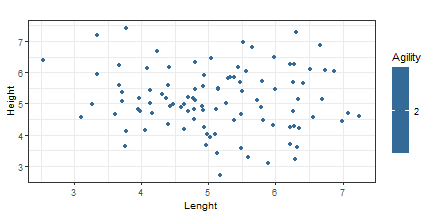
\includegraphics{Q1_files/figure-latex/Figure2-1} 

}

\caption{Caption Here \label{Figure2}}\label{fig:Figure2-1}
\end{figure}
\begin{figure}[H]

{\centering 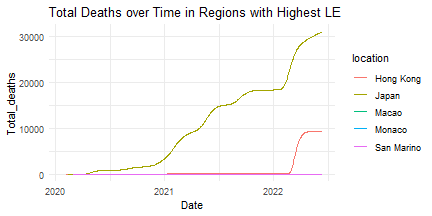
\includegraphics{Q1_files/figure-latex/Figure2-2} 

}

\caption{Caption Here \label{Figure2}}\label{fig:Figure2-2}
\end{figure}

\begin{verbatim}
## # A tibble: 5 x 2
##   location                 average_life_expectancy
##   <chr>                                      <dbl>
## 1 Central African Republic                    53.3
## 2 Chad                                        54.2
## 3 Lesotho                                     54.3
## 4 Nigeria                                     54.7
## 5 Sierra Leone                                54.7
\end{verbatim}

\begin{figure}[H]

{\centering 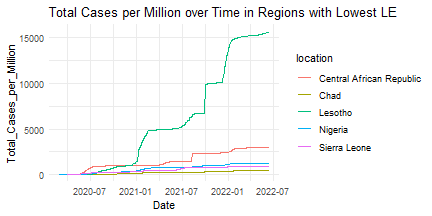
\includegraphics{Q1_files/figure-latex/Figure2-3} 

}

\caption{Caption Here \label{Figure2}}\label{fig:Figure2-3}
\end{figure}
\begin{figure}[H]

{\centering 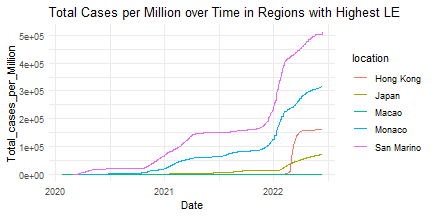
\includegraphics{Q1_files/figure-latex/Figure2-4} 

}

\caption{Caption Here \label{Figure2}}\label{fig:Figure2-4}
\end{figure}

Show how quickly different regions increased their hospitalization
facilities, and whether this led or lagged ICU admissions.

Hospitalisation and ICU admission are plotted.

Plotting across continent, we can see that each continent experienced
waves of hospitalisation at different times. Europe, North America and
Asia experienced the highest shocks in hospitalisations. Hospitalisation
in Africa were always low.

Europe and South America experienced the highest numbers of weekly ICU
admission per million . This is interesting because South America did
not have as sharp spikes in general hospitalisations compared to other
continents.

Plotting hospital patients and ICU patients, it can be seen that they
follow the same trends and waves. ICU patient numbers always increase
globally when global hospitalisations increase. Therefore,
hospitalisation led ICU hospitalisation.

We can also see that there is a positive correlation (0.6) between the
numberr of hospital patients and number of tests. Therefore, the number
of tests conducted can act as a good indicator of hospitalisation.

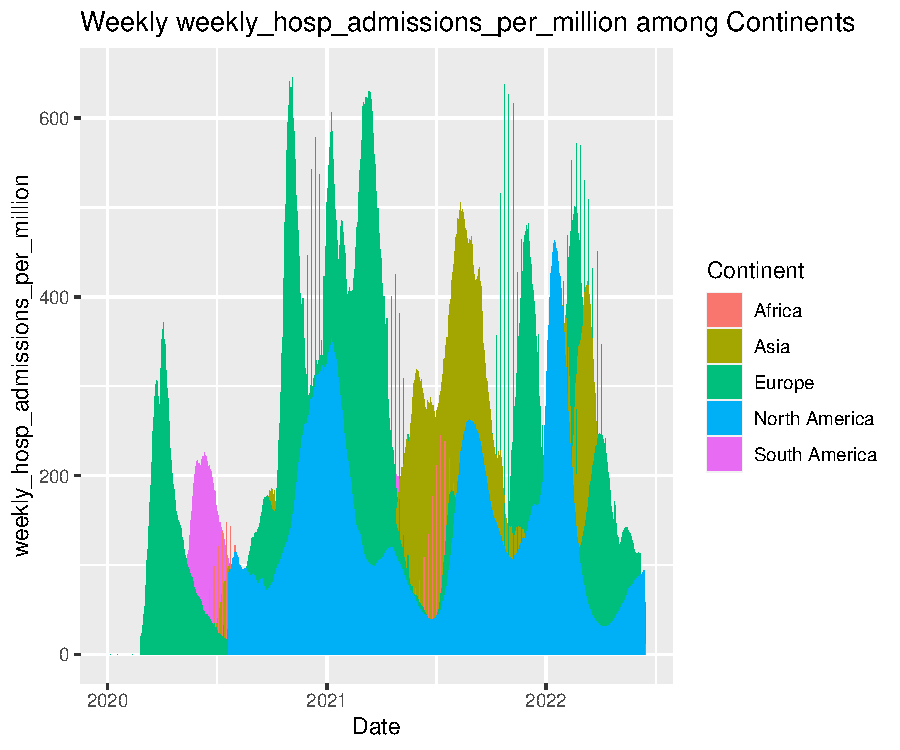
\includegraphics{Q1_files/figure-latex/unnamed-chunk-2-1.pdf}

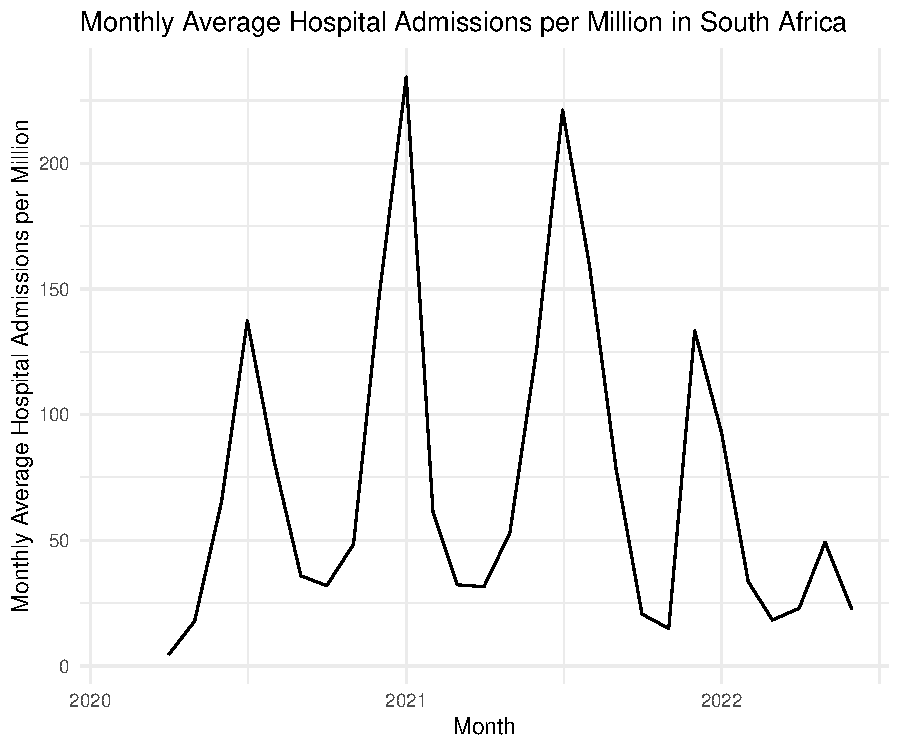
\includegraphics{Q1_files/figure-latex/unnamed-chunk-3-1.pdf}
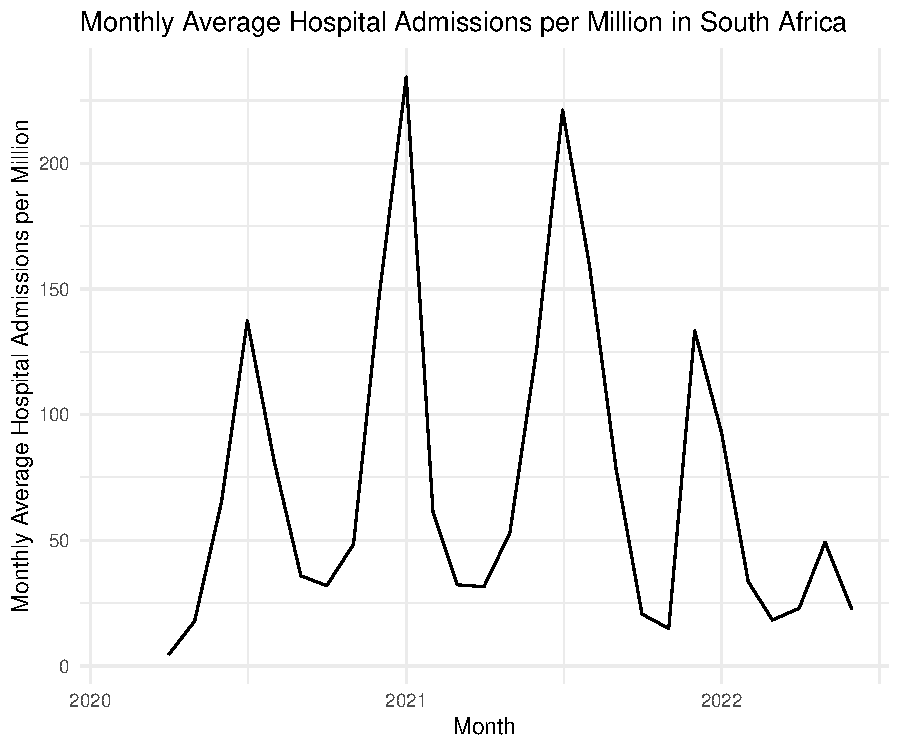
\includegraphics{Q1_files/figure-latex/unnamed-chunk-3-2.pdf}

\begin{verbatim}
## [1] 0.6159445
\end{verbatim}

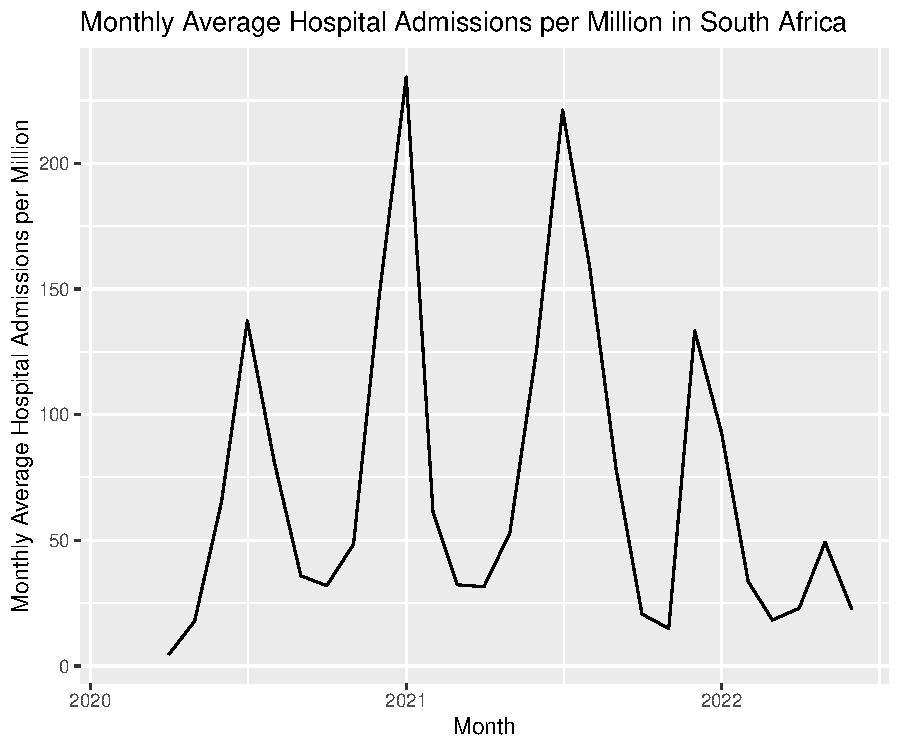
\includegraphics{Q1_files/figure-latex/unnamed-chunk-3-3.pdf}

\hfill

\hypertarget{conclusion}{%
\section{Conclusion}\label{conclusion}}

In conclusion, Covid-19 wrecked havoc throughout the world, leading to
increase deaths and hospitalisations.

\newpage

\bibliography{Tex/ref}





\end{document}
